%! Author = mdh81
%! Date = 7/27/23

\documentclass{article}
\usepackage{amsmath}
\usepackage{mathtools}
\usepackage{graphicx}

\newcommand{\xaxis}{
    \begin{bmatrix}
        1 \\
        0 \\
        0 \\
    \end{bmatrix}
}

\newcommand{\yaxis}{
    \begin{bmatrix}
        0 \\
        1 \\
        0 \\
    \end{bmatrix}
}

\newcommand{\zaxis}{
    \begin{bmatrix}
        0 \\
        0 \\
        1 \\
    \end{bmatrix}
}

\newcommand{\rotAxis}{
    \begin{bmatrix}
        R_x \\
        R_y \\
        R_z \\
    \end{bmatrix}
}

\newcommand{\vparallelForX}{
    \xaxis . \rotAxis 
    \rotAxis
}

\newcommand{\vparallelForY}{
    \yaxis . \rotAxis 
    \rotAxis
}

\newcommand{\vparallelForZ}{
    \zaxis . \rotAxis 
    \rotAxis
}

\begin{document}

    \begin{center}
        \section*{Rotation About Arbitrary Axis}
    \end{center}

    \subsection*{Derivation for the rotation equation}
    
    In this section we will derive the equation to rotate a vector $V$ about another vector $R$ in 3D space. Vector $V$'s projection
    on vector $R$ is

    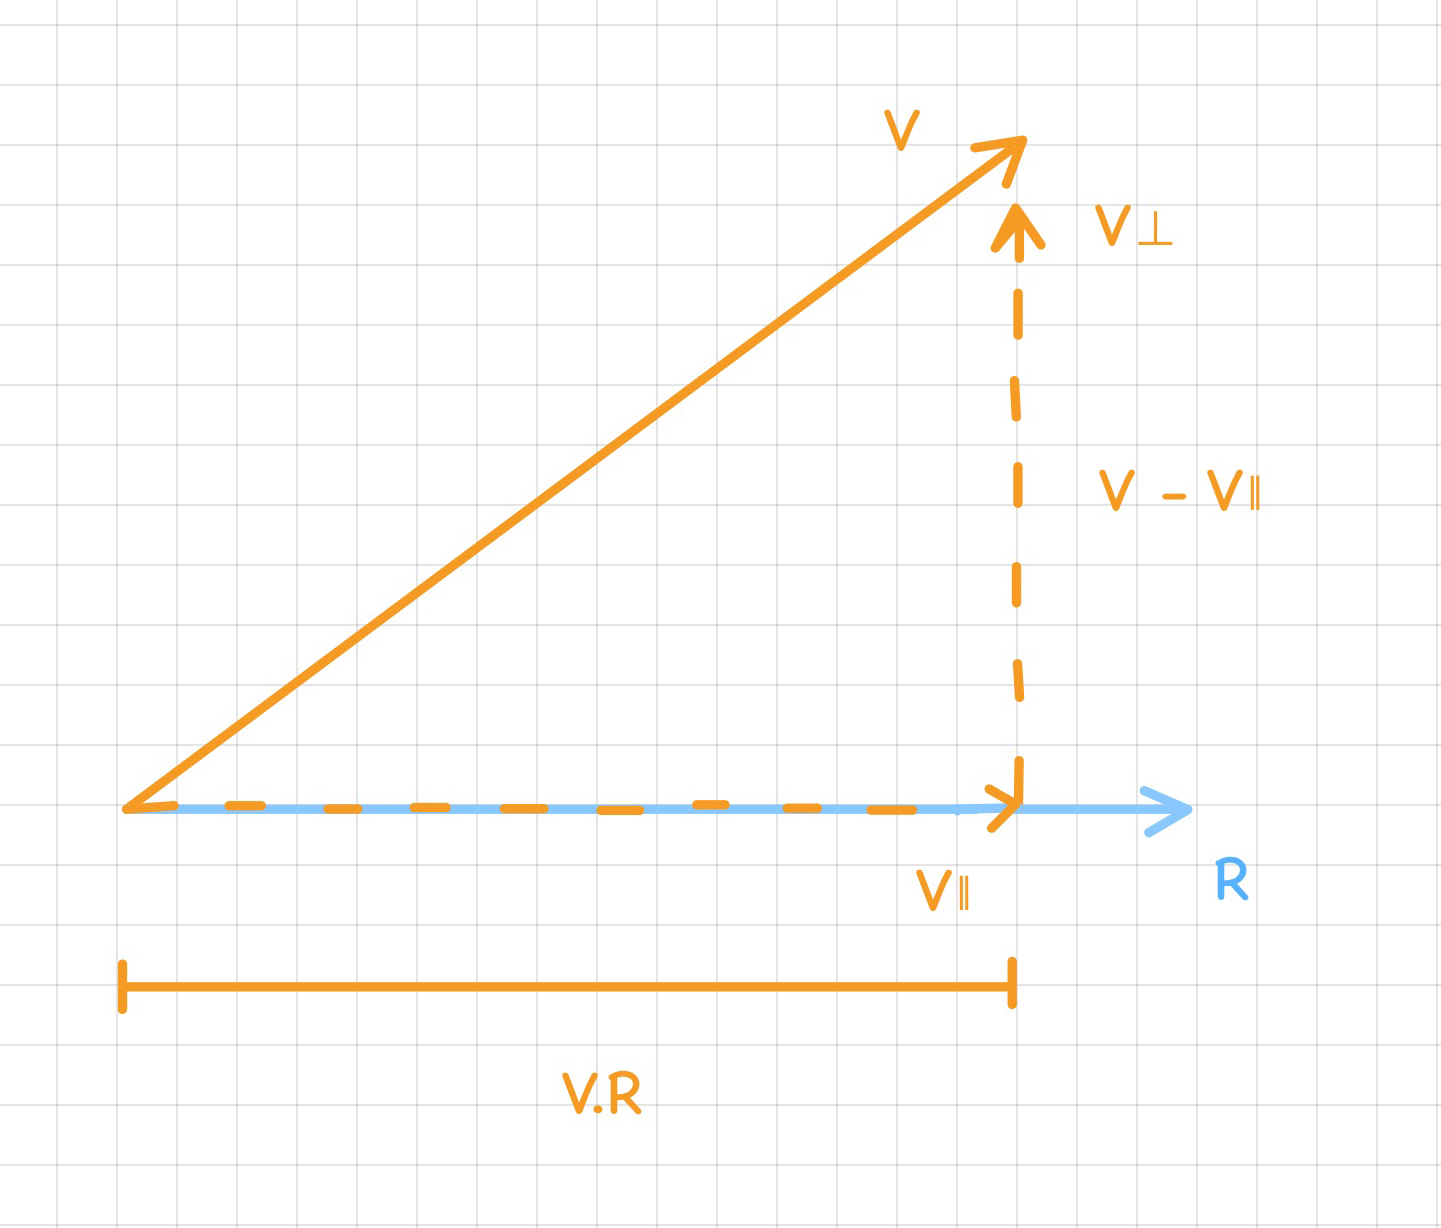
\includegraphics[width=0.75\textwidth]{../images/VectorProjection.jpg}

    \noindent We split $V$ into two vector components $V_{\parallel}$ and $V_{\perp}$ that are parallel and perpendicular to $R$, respectively.

    \begin{align}
        V &= V_{\parallel} + V_{\perp} \\
        V_{\parallel} &= (V.R) R \label{eq:vparallel} \\
        V_{\perp} &= V - (V.R) R \label{eq:vperp}
    \end{align}

    We can describe the rotation of $V$ in the plane perpendicular to $R$

    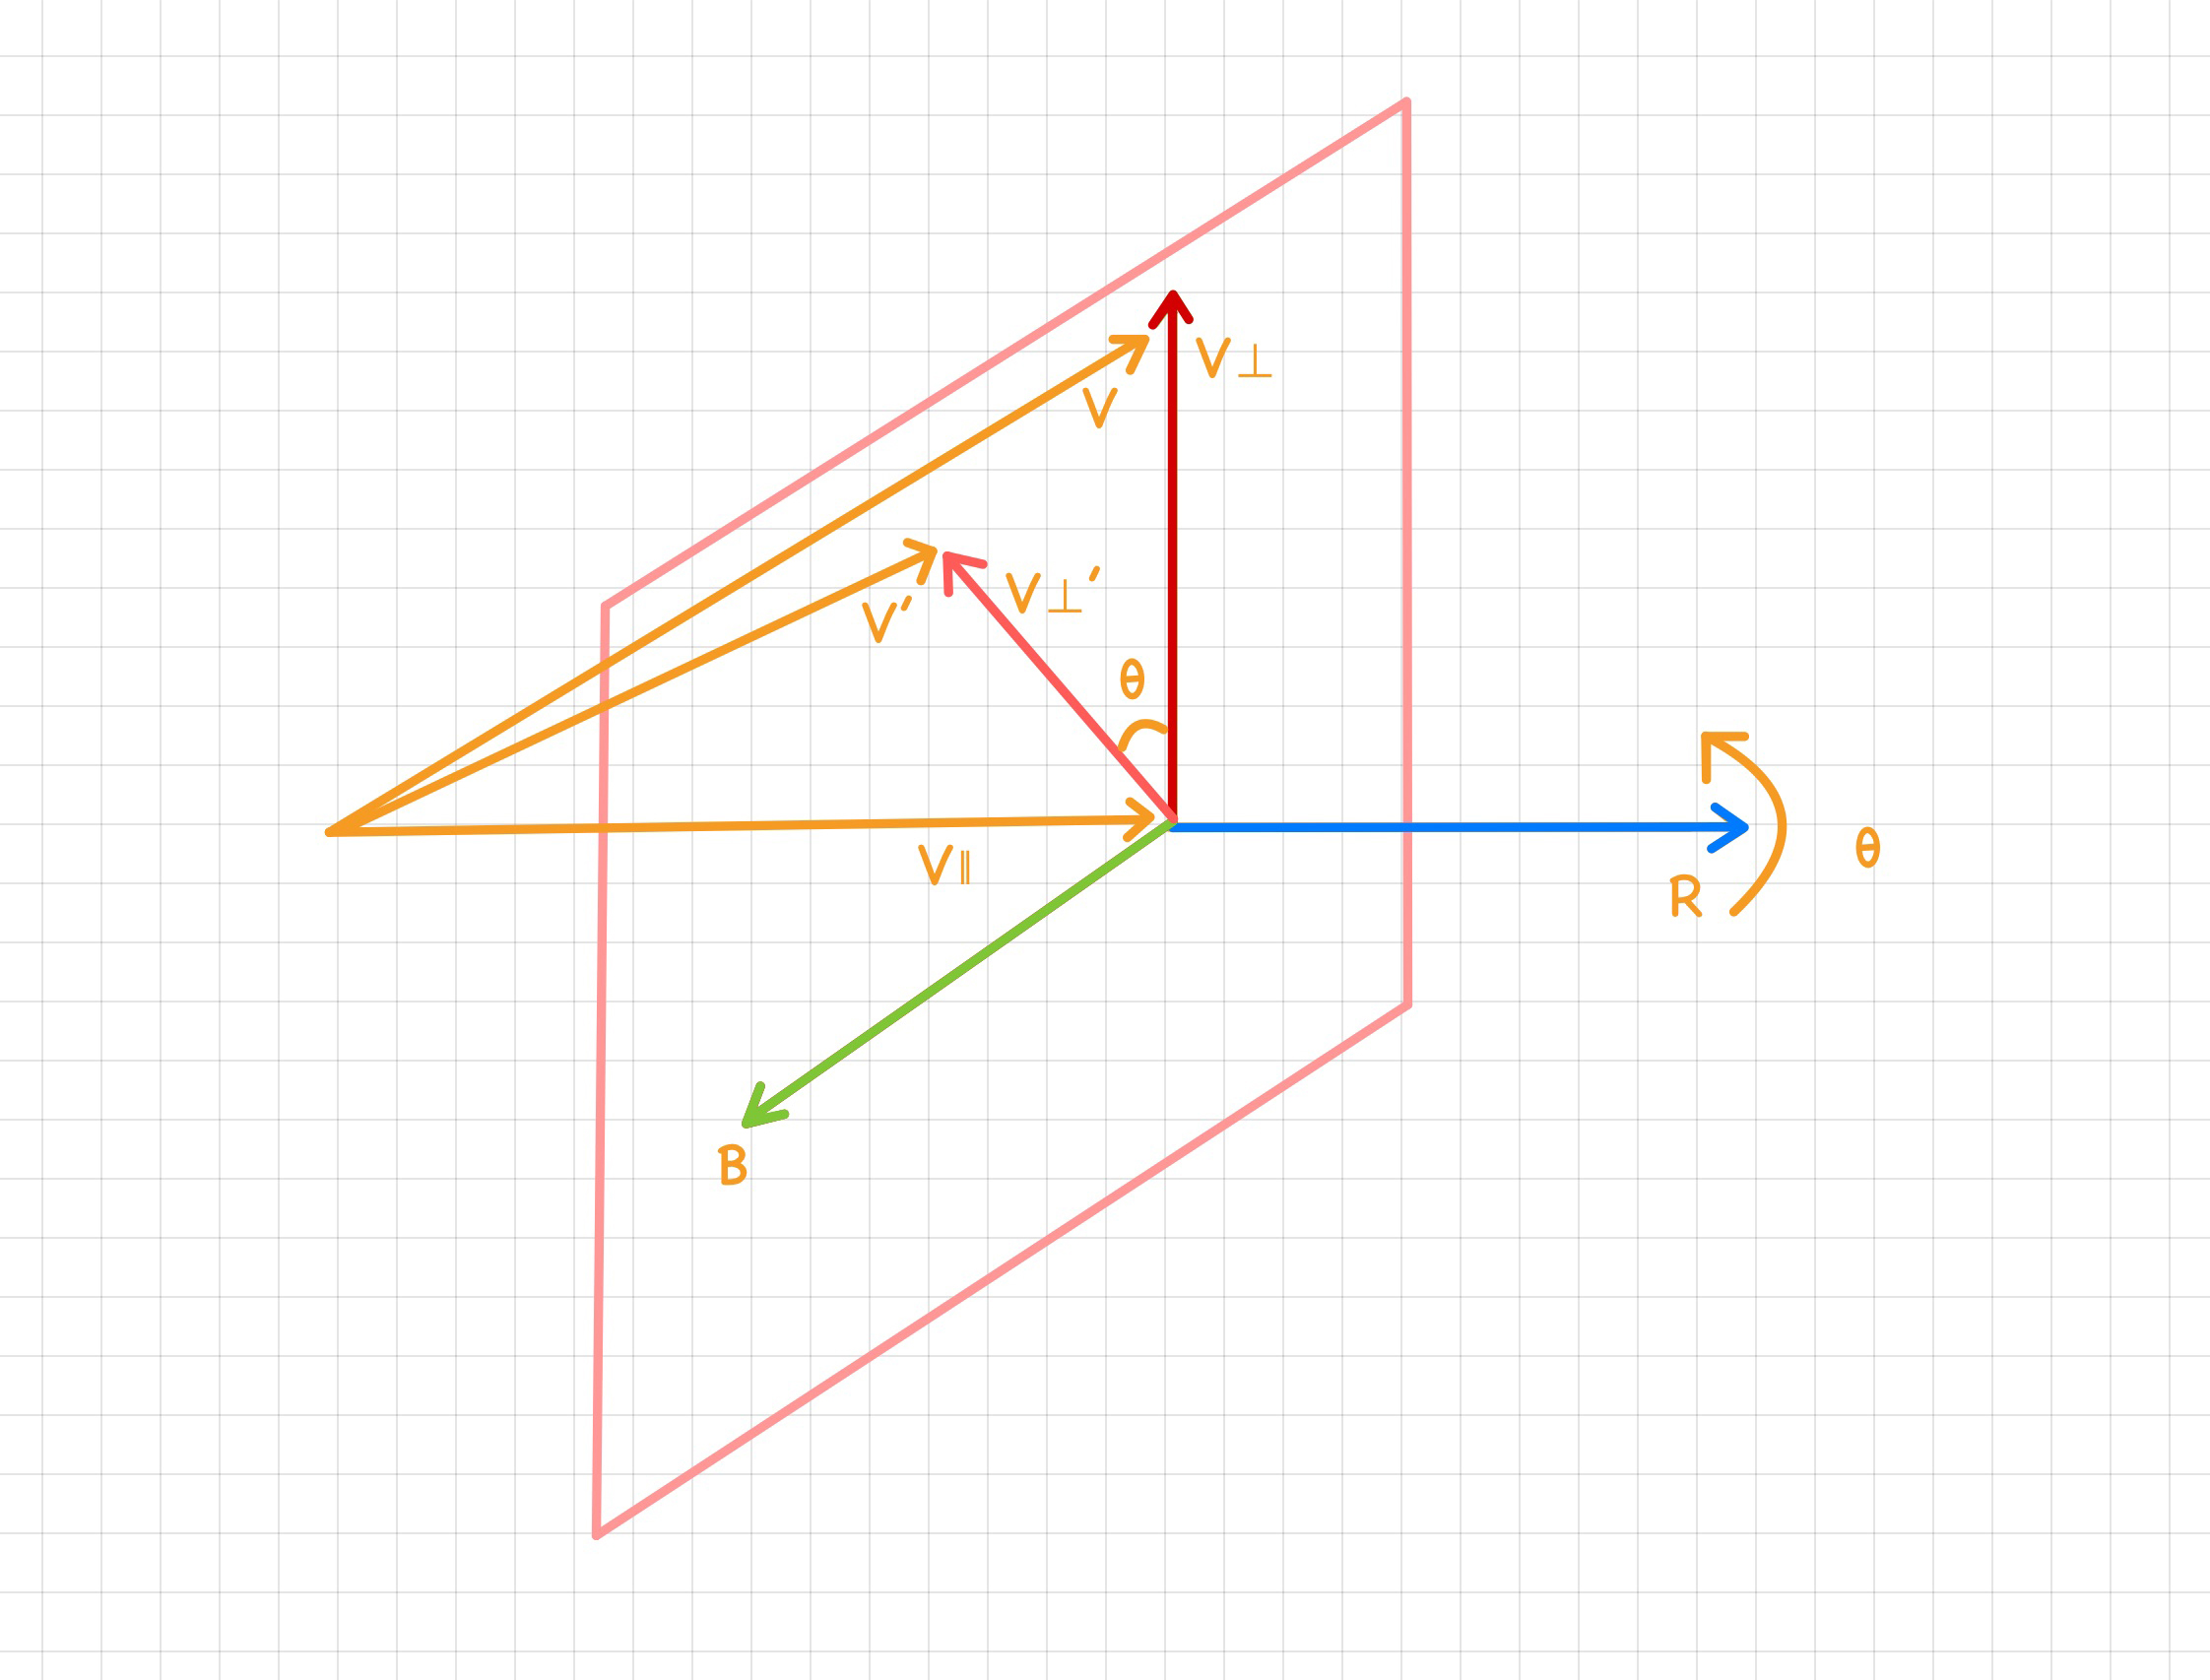
\includegraphics[width=0.75\textwidth]{../images/Rotation_About_ArbitraryAxis.jpg}

    \noindent We can see when $V$ is rotated about $R$ by $\theta$, the resulting vector is $V'$. Considering the vector projection of $V'$ on $R$
    
    \begin{align}
        V' &= V'_{\parallel} + V'_{\perp} \\
        \intertext{Because $V'_{\parallel} = V_{\parallel}$}
        V' &= V_{\parallel} + V'_{\perp} \\
        \intertext{Substituting $V_{\parallel}$ from \ref{eq:vparallel}}
        V' &= (V.R) R + V'_{\perp} \label{eq:vdash}
    \end{align}

    \noindent{$V$ and $R$ are known quantities. $V'{\perp}$ can be calculated by observing that {$V_{\perp}$ and $B$ and are two 
            mutually perpendicular plane vectors. Along with $R$ they describe a coordinate frame, $V{\perp}BR$ that can be used
            to compute $V'_{\perp}$}. Since $B$ is mutally perpendicular to $V'{\perp}$ and $R$, it can be expressed as}
    
        \begin{align}
        B &= R \times V_{\perp} \\
        \intertext{Substituting $V_{\perp}$ from \ref{eq:vperp}}
        B &= R \times (V - V_{\parallel}) \\
        \intertext{Since cross product distributes over vector subtraction and since $V_{\parallel}$ and $R$ are parallel}
        B &= R \times V - R \times V_{\parallel} \\
        B &= R \times V - 0 \\
        B &= R \times V \label{eq:b} \\
        \intertext{Using $V_{\perp}$ and $B$ as basis vectors, $V'_{\perp}$ can be written as}
        V'_{\perp} &= V_{\perp} cos\theta + (R \times V) sin\theta \\
        \intertext{Substituting $V'{\perp}$ into the equation \ref{eq:vdash}, we get the final equation for $V'$ in terms of $V$ and $R$}
        V' &= (V.R) R + V_{\perp} cos\theta + (R \times V) sin\theta \\ 
        V' &= (V.R) R + (V - (V.R) R) cos\theta + (R \times V) sin\theta \label{eq:rotEq}
    \end{align}
    
    \subsubsection*{Note}
    \noindent There are three terms in \ref{eq:rotEq} 

    \begin{align}
        T1 &= (V.R) R \\
        T2 &= (V - (V.R) R) cos\theta \\
        T3 &= (R \times V) sin\theta
    \end{align}

    \noindent Notice that $T2$ is actually $(V-T1) cos\theta$. We will be using these three terms in the derivation of the rotation matrix in the next section


    \subsection*{Derivation for the rotation matrix}

    A column-major rotation matrix is of the form
    \[
        \begin{bmatrix}
            B1 & B2 & B3
        \end{bmatrix}
    \]

    \noindent The columns $B1$,$B2$, and $B3$ are the coordinates of the basis vectors after rotation. To derive the rotation matrix for rotating $V$ and producing $V'$, we start with the basis vectors of the right-handed coordinate system

    \[
        \begin{bmatrix}
            1 & 0 & 0 \\
            0 & 1 & 0 \\
            0 & 0 & 1
        \end{bmatrix}
    \]

    \noindent We first rotate these basis vectors using the rotation equation (12), and to form the rotation matrix, we add the rotated coordinates of the basis vectors to the rotation matrix

    \subsubsection*{Rotation of X-axis}

    Substituting x-axis for $V$ in \ref{eq:rotEq}, we can get the $B1$ vector after rotation. Instead of solving for $V'$ in one-shot, for simplicity's sake we will solve the three terms $T1,T2, and T3$ separately and assemble the results 
   
    \begin{align}
        T1 &= \vparallelForX \\
        T2 &= \xaxis - \vparallelForX cos\theta \\
        T3 &= \rotAxis \times \xaxis sin\theta 
    \end{align}

    Solving for $T1$
    \begin{align}
        T1 &= \vparallelForX \\
        T1 &= R_x \rotAxis \\
        T1 &= \begin{bmatrix} R_x^2 \\ R_xR_y \\ R_xR_z \end{bmatrix}
    \end{align}

    Solving for $T2$
    \begin{align}
        T2 &= \xaxis - \vparallelForX sin\theta \\
        T2 &= \begin{bmatrix} 1-R_x^2 \\ -R_xR_y \\ -R_xR_z \end{bmatrix} cos\theta \\
        T2 &= \begin{bmatrix} (1-R_x^2)cos\theta \\ -R_xR_ycos\theta \\ -R_xR_zcos\theta \end{bmatrix}
    \end{align}

    Solving for $T3$
    \begin{align}
        T3 &= \rotAxis \times \xaxis sin\theta \\
        T3 &= \begin{bmatrix} 0\\ R_z \\ -R_y \end{bmatrix}sin\theta\\
        T3 &= \begin{bmatrix} 0 \\ R_zsin\theta \\ -R_ysin\theta \end{bmatrix}
    \end{align}
    
    Summing the terms 

    \begin{align}
        V' &= 
        \begin{bmatrix} R_x^2 \\ R_xR_y \\ R_xR_z \end{bmatrix} +  
        \begin{bmatrix} (1-R_x^2)cos\theta \\ -R_xR_ycos\theta \\ -R_xR_zcos\theta \end{bmatrix} + 
        \begin{bmatrix} 0 \\ R_zsin\theta \\ -R_ysin\theta \end{bmatrix} \\
        V' &= 
        \begin{bmatrix}
            R_x^2 + (1-R_x^2)cos\theta \\ 
            R_xR_y - R_xR_ycos\theta + R_zsin\theta \\ 
            R_xR_z - R_xR_zcos\theta -R_ysin\theta  
        \end{bmatrix} \\
        V' &= 
        \begin{bmatrix}
            R_x^2(1 - cos\theta) + cos\theta \\ 
            R_xR_y(1 - cos\theta) + R_zsin\theta \\ 
            R_xR_z(1 - cos\theta) - R_ysin\theta  
        \end{bmatrix} \label{eq:xaxisAfterRotation} 
    \end{align}

    \subsubsection*{Rotation of Y-axis}

    Terms $T1,T2, and T3$ for $\yaxis$ is 

    \begin{align}
        T1 &= \vparallelForY \\
        T2 &= \yaxis - \vparallelForY cos\theta \\
        T3 &= \rotAxis \times \yaxis sin\theta 
    \end{align}

    Solving for $T1$
    \begin{align}
        T1 &= \vparallelForY \\
        T1 &= R_y \rotAxis \\
        T1 &= \begin{bmatrix} R_xR_y \\ R_y^2 \\ R_yR_z \end{bmatrix} 
    \end{align}
    
    Solving for $T2$
    \begin{align}
        T2 &= \yaxis - \vparallelForY cos\theta \\
        T2 &= \begin{bmatrix} -R_xR_y \\ (1-R_y^2) \\ -R_yR_z \end{bmatrix} cos\theta \\
        T2 &= \begin{bmatrix} -R_xR_ycos\theta \\ (1-R_y^2)cos\theta \\ -R_yR_zcos\theta \end{bmatrix}
    \end{align}

    Solving for $T3$
    \begin{align}
        T3 &= \rotAxis \times \yaxis sin\theta \\
        T3 &= \begin{bmatrix} -R_z \\ 0 \\ R_x \end{bmatrix}sin\theta\\
        T3 &= \begin{bmatrix} -R_zsin\theta \\ 0 \\ R_xsin\theta \end{bmatrix}
    \end{align}

    Summing the terms 

    \begin{align}
        V' &= 
        \begin{bmatrix} R_xR_y \\ R_y^2 \\ R_yR_z \end{bmatrix} +  
        \begin{bmatrix} -R_xR_ycos\theta \\ (1-R_y^2)cos\theta \\ -R_yR_zcos\theta \end{bmatrix}
        \begin{bmatrix} -R_zsin\theta \\ 0 \\ R_xsin\theta \end{bmatrix}
        \begin{bmatrix} 0 \\ R_zsin\theta \\ -R_ysin\theta \end{bmatrix} \\
        V' &= 
        \begin{bmatrix}
            R_xR_y - R_xR_ycos\theta -R_zsin\theta \\ 
            R_y^2 + cos\theta -R_y^2cos\theta \\ 
            R_yR_z - R_zR_ycos\theta + R_xsin\theta  
        \end{bmatrix} \\
        V' &= 
        \begin{bmatrix}
            R_xR_y(1 - cos\theta) - R_zsin\theta \\ 
            R_y^2(1 - cos\theta) + cos\theta \\ 
            R_yR_z(1 - cos\theta) + R_xsin\theta  
        \end{bmatrix} \label{eq:yaxisAfterRotation}
    \end{align}

    \subsubsection*{Rotation of Z-axis}

    Terms $T1,T2, and T3$ for $\zaxis$ is 

    \begin{align}
        T1 &= \vparallelForZ \\
        T2 &= \zaxis - \vparallelForZ cos\theta \\
        T3 &= \rotAxis \times \zaxis sin\theta 
    \end{align}

    Solving for $T1$
    \begin{align}
        T1 &= \vparallelForZ \\
        T1 &= R_z \rotAxis \\
        T1 &= \begin{bmatrix} R_xR_z \\ R_yR_z \\ R_zR_z \end{bmatrix} 
    \end{align}
    
    Solving for $T2$
    \begin{align}
        T2 &= \zaxis - \vparallelForZ cos\theta \\
        T2 &= \begin{bmatrix} -R_xR_z \\ -R_yR_z \\ (1-R_z^2) \end{bmatrix} cos\theta \\
        T2 &= \begin{bmatrix} -R_xR_zcos\theta \\ -R_yR_zcos\theta \\ (1-R_z^2)cos\theta \end{bmatrix}
    \end{align}

    Solving for $T3$
    \begin{align}
        T3 &= \rotAxis \times \zaxis sin\theta \\
        T3 &= \begin{bmatrix} R_y \\ -R_x \\ 0 \end{bmatrix}sin\theta\\
        T3 &= \begin{bmatrix} R_ysin\theta \\ -R_xsin\theta \\ 0 \end{bmatrix}
    \end{align}

    Summing the terms 

    \begin{align}
        V' &= 
        \begin{bmatrix} R_xR_z \\ R_yR_z \\ R_z^2 \end{bmatrix} +  
        \begin{bmatrix} -R_xR_zcos\theta \\  -R_yR_zcos\theta \\ (1-R_z^2)cos\theta \end{bmatrix}
        \begin{bmatrix} R_ysin\theta \\ -R_xsin\theta \\ 0 \end{bmatrix} \\
        V' &= 
        \begin{bmatrix}
            R_xR_z - R_xR_zcos\theta + R_ysin\theta \\ 
            R_yR_z - R_yR_zcos\theta - R_xsin\theta \\ 
            R_z^2  + (1-R_z^2)cos\theta   
        \end{bmatrix} \\
        V' &= 
        \begin{bmatrix}
            R_xR_z(1 - cos\theta) + R_ysin\theta \\ 
            R_yR_z(1 - cos\theta) - R_xsin\theta \\ 
            R_z^2(1 - cos\theta) + cos\theta  
        \end{bmatrix} \label{eq:zaxisAfterRotation}
    \end{align}


    \noindent Finally, assembling the three transformed basis vectors into the rotation matrix we get the matrix that transforms any arbitrary vector about a different arbitrary vector $R$
    
    \begin{align}
        \begin{bmatrix}
            \begin{matrix}
                R_x^2(1 - cos\theta) + cos\theta \\ 
                R_xR_y(1 - cos\theta) + R_zsin\theta \\ 
                R_xR_z(1 - cos\theta) - R_ysin\theta  
            \end{matrix}
            \begin{matrix}
                R_xR_y(1 - cos\theta) - R_zsin\theta \\ 
                R_y^2(1 - cos\theta) + cos\theta \\ 
                R_yR_z(1 - cos\theta) + R_xsin\theta  
            \end{matrix}
            \begin{matrix}
                R_xR_z(1 - cos\theta) + R_ysin\theta \\ 
                R_yR_z(1 - cos\theta) - R_xsin\theta \\ 
                R_z^2(1 - cos\theta) + cos\theta  
            \end{matrix}
        \end{bmatrix}
    \end{align}


\end{document}

